\documentclass{article}
\usepackage[utf8]{inputenc}
\usepackage{geometry}
\usepackage{graphicx}
\usepackage{url,hyperref}
\hypersetup{colorlinks,citecolor=red,urlcolor=blue} 

\title{
	Web Information Extraction and Retrieval\\
	Programming Assignment 1: \\
	Crawler implementation
}

\author{
  Marko Prelevikj\\
  63130345\\
  \texttt{mp2638@student.uni-lj.si}
  \and
  Gojko Hajduković\\
  63180431\\
  \texttt{gh8590@student.uni-lj.si}
  \and
  Stefan Ivanišević\\
  63170405\\
  \texttt{si0539@student.uni-lj.si}
}
\date{April 2019}

\begin{document}

\maketitle

\section{Introduction}

\section{Implementation specifics}
The implementation of the web crawler is done in Scala, which is a functional programming language, offering a lot of syntactical sugars which make the development process easier.
We chose it in order to improve our programming skills in Scala, and also, learn a lot about its capabilities for concurrent programming.

\subsection{Dependencies}
To make the development process as easy as possible, we are using a number of dependencies. In this report, we are listing the once which are most significant, whilst the list of entire dependencies is available in the \texttt{build.sbt} file. 
\begin{itemize}
	\item \texttt{akka-actor} - providing us with the support of multi-threading through the concept of actor systems~\cite{Akka:ActorSystem}.
	\item \texttt{slick} - a functional relational mapping library to easily store data into the database~\cite{Slick}.
	\item \texttt{crawler-commons} - a library containing common utilities for crawlers~\cite{Crawler-commons}.
	\item \texttt{htmlunit} - headless browser which renders the html content of a provided URL~\cite{htmlunit}.
	\item \texttt{bigqueue} - a multithread-safe persistent queue for keeping the frontier~\cite{bigqueue}.
	\item \texttt{JSoup} - a library for HTML document parsing~\cite{jsoup}.
\end{itemize}

\subsection{Database modifications}
In order to make the implementation more insightful, we expanded the initial database with additional columns as follows:
\subsubsection{Table \texttt{page}}
We introduced the fields:
\begin{itemize}
    \item \texttt{hash} - SHA256 hash of the entire HTML content of the page, used for duplicate detection.
    \item \texttt{load\_time} - time needed to load the page
    \item \texttt{stored\_time} - when the page was added in the queue
\end{itemize}
\subsubsection{Table \texttt{page\_type}}
We introduced the following values:
\begin{itemize}
    \item \texttt{INVALID} - in case there has occurred an unknown error while loading the page
    \item \texttt{DISALLOWED} - if the page is not allowed by the \texttt{robots.txt} file
\end{itemize}

\subsubsection{Table \texttt{page\_data}}
We introduced the following column:
\begin{itemize}
    \item \texttt{filename} - canonical url of the stored file
\end{itemize}

\subsubsection{Storing process}
We altered the storing process as well. We omit a page entry of the type \textit{BINARY} which should be a reference to the \textit{image} or \textit{page\_data} table. Instead, we are linking the resources directly to the pages where they occurred. For example, if there had been an image linked to a page with \texttt{id = 1}, we enter an image entry with a reference to the page with \texttt{id = 1}.

\section{Crawler implementation}
The development process of the crawler was done in multiple iterations. In the first iteration, we developed all the required utilities to build the crawler upon. These utilities include: URL-canonicalization, \texttt{SiteMap} parsing, \texttt{robots.txt} parsing, database service to store the obtained data. Furthermore, we developed the core concepts, and the basic pipeline of how the crawler should interact with the frontier and the database. Finally, we created workers which are going to perform the crawling.

\subsection{Core concepts}
The following steps describe the process of fetching and storing the data retrieved from a given URL.
\begin{enumerate}
	\item frontier dequeueing - get the next page from the frontier
	\item \texttt{robots.txt} check - check whether the page is allowed in the \texttt{robots.txt}, skip it if not. If the \texttt{robots.txt} is missing - allow it by default
	\item page rendering - get the page content and HTTP status code using \texttt{HtmlUnit}
	\item data extraction - extract all the detected links pages and binary data in the page using \texttt{JSoup}
	\item data deduplication - detect the entries which already exist, and link them accordingly. 
	\item data storage - The duplicate detection is performed on a database level: if the URL exists - it is a duplicate, if it does not, it checks whether its hash code already exists, if it does not it is finally written into the database.
	\item frontier enqueueing - All the non-duplicate links, images, and binary data is enqueued in the frontier to be processed when they come in line.
	\item delay - after all the processing has been performed, the worker waits for at least \texttt{5s} until the next page is processed, depending on the presence of \texttt{robots.txt}.
	\item repeat the process for the rest of the entries
\end{enumerate}

\subsection{Version 1 - jittered delay}

Figure~\ref{fig:1}


\subsection{Version 2 - Distributed BF}
Figure~\ref{fig:2}


\begin{figure}
	\begin{minipage}{0.45\textwidth}
		\centering
		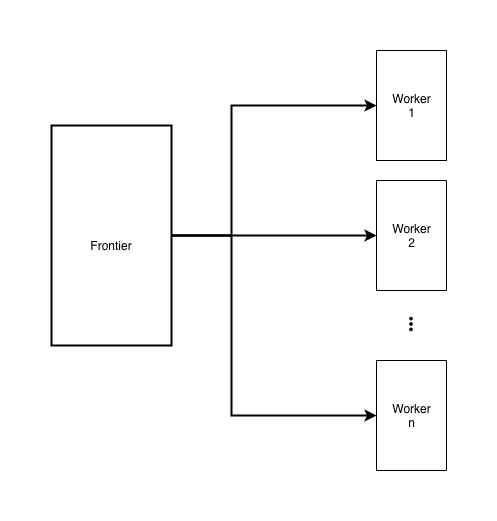
\includegraphics[width=0.9\textwidth]{jittered-delay.png}
		\caption{V1.}
		\label{fig:1}
	\end{minipage}\hfill
	\begin{minipage}{0.45\textwidth}
		\centering
		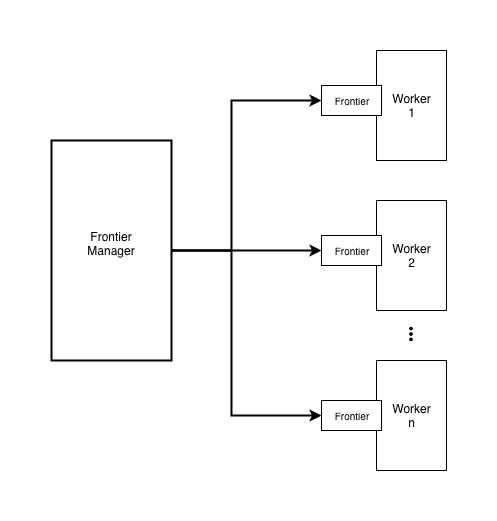
\includegraphics[width=0.9\textwidth]{frontier-manager.png}
		\caption{V2.}
		\label{fig:2}
\end{minipage}
\end{figure}


\section{Data Analysis}

\subsection{Experiment 1 - Pages only with initial seed}
\subsection{Experiment 2 - Provided seed all data}
\subsection{Experiment 3 - Extended seed all data}
binary data is ignored completely
\section{Conclusion}

% SELECT count(*), clock_timestamp() FROM page;
% SELECT count(*), clock_timestamp() FROM link;
% SELECT count(*), clock_timestamp() FROM image;
% SELECT count(*), clock_timestamp() FROM page_data;

\bibliographystyle{IEEEtran}
\bibliography{refs}

\end{document}
